\documentclass[11pt, spanish, a4paper, twopage]{article}
% LTeX: language=es-AR

% Versión 1.er cuat 2021 Víctor Bettachini < vbettachini@unlam.edu.ar >

\usepackage[T1]{fontenc}
\usepackage[utf8]{inputenc}

\usepackage[spanish, es-tabla]{babel}
% \def\spanishoptions{argentina} % Was macht dass?
% \usepackage{babelbib}
% \selectbiblanguage{spanish}
% \addto\shorthandsspanish{\spanishdeactivate{~<>}}


\usepackage{graphicx}
\graphicspath{{./figuras/}{../LaTeX/}{../figurasLaTeX/}{./figs}}
% \usepackage{float}

\usepackage[arrowdel]{physics}
\newcommand{\pvec}[1]{\vec{#1}\mkern2mu\vphantom{#1}}
% \usepackage{units}
\usepackage[separate-uncertainty= true, multi-part-units= single, range-units= single, range-phrase= {~a~}, locale= FR]{siunitx}
\usepackage{isotope} % $\isotope[A][Z]{X}\to\isotope[A-4][Z-2]{Y}+\isotope[4][2]{\alpha}

\usepackage{tasks}
\usepackage[inline]{enumitem}
% \usepackage{enumerate}

\usepackage{hyperref}

% \usepackage{amsmath}
% \usepackage{amstext}
% \usepackage{amssymb}

\usepackage{tikz}
\usepackage{tikz-3dplot}
\usepackage{tikz-dimline}
\usetikzlibrary{calc}
% \usetikzlibrary{math}
\usetikzlibrary{arrows.meta}
\usetikzlibrary{snakes}
\usetikzlibrary{decorations}
\usetikzlibrary{decorations.pathmorphing}
\usetikzlibrary{patterns}

\usepackage[hmargin=1cm,vmargin=3cm, top= 0.75cm,nohead]{geometry}

\usepackage{lastpage}
\usepackage{fancyhdr}
\pagestyle{fancyplain}
\fancyhf{}
\setlength\headheight{28.7pt} 
\fancyhead[LE, LO]{\textbf{Mecánica Analítica Computacional} }
% \fancyhead[LE, LO]{\textbf{Mecánica General} }
\fancyhead[RE, RO]{\href{https://ingenieria.unlam.edu.ar/}{$\vcenter{\hbox{
\includegraphics[height=1cm]{ambos.pdf}}}$}}
\fancyfoot{\href{https://creativecommons.org/licenses/by-nc-sa/4.0/deed.es_ES}{$\vcenter{\hbox{
\includegraphics[height=0.4cm]{by-nc-sa_80x15.pdf}}}$} \href{https://ingenieria.unlam.edu.ar/}{DIIT - UNLaM}}
\fancyfoot[C]{ {\tiny Actualizado al \today} }
\fancyfoot[RO, LE]{Pág. \thepage/\pageref{LastPage}}
\renewcommand{\headrulewidth}{0pt}
\renewcommand{\footrulewidth}{0pt}

% LTeX: language = es-AR

\begin{document}
\begin{center}
%	\textsc{\large Mecánica general}\\
	\textsc{\large Vibraciones | Único grado de libertad}
\end{center}

% De poder resolver estos problemas en forma autónoma puede asumir que adquirió los conocimientos mínimos sobre los temas abordados en la semana. No dude en consultar a docentes y compañeros si no puede terminarlos. Los problemas marcados con * son opcionales.

\begin{enumerate}

				
\item 
\begin{minipage}[t][4cm]{0.65\textwidth}
	\textbf{Péndulo restringido}
	El sistema mostrado en la figura consiste en una masa $m$ y una barra rígida de longitud $l$, cuya masa se desprecia.
	El sistema está restringido por dos resortes de coeficiente de rigidez $k_1$ y $k_2$.

	Obtenga la ecuación de la dinámica asumiendo pequeñas oscilaciones y la frecuencia natural de oscilación del sistema.
\end{minipage}
\begin{minipage}[c][3cm][t]{0.3\textwidth}
	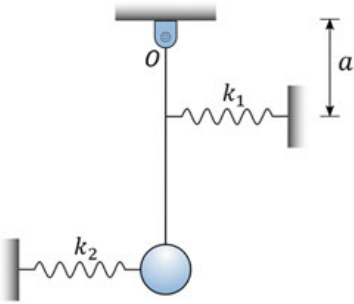
\includegraphics[width=\textwidth]{shabana_fig_P1_1.png}
\end{minipage}



\item 
\begin{minipage}[t][6cm]{0.65\textwidth}
	\textbf{Audi TT Coupé}
	En la figura se muestra la ubicación de los amortiguadores de un \emph{Audi TT Coupé}.
	Las \href{https://media.audiusa.com/assets/documents/original/8253-FINAL2021TTTechSpecs.pdf}{especificaciones de esta máquina} indican que con un pasajero y 90\% de carga de nafta tiene un peso de \SI{1450}{\kilo\gram}.
	% Las \href{https://www.audi.de/de/brand/de/neuwagen/tt/tt-coupe.html#layer=/de/brand/de/neuwagen/tt/tt-coupe.engine_compare.fvp09g_0.techdata.html}{especificaciones de esta máquina} indican que con un pasajero y 90\% de carga de nafta tiene un peso de \SI{1370}{\kilo\gram}.

	Utilice el modelo de cuarto de coche (\emph{quarter car model}), en el que se asume que cada amortiguador soporta un cuatro del peso.
	Simplificará aún más este modelo eliminando el neumático, tanto su masa y su capacidad de operar como amortiguador, para encargar esta última tarea únicamente en la suspensión.

	Puesto que manejar en el régimen de sobre-amortiguación es incómodo, pues tras un bache puede producirse un violento rebote, debe ajustar la suspensión en consecuencia.
	De un \href{https://journals.sagepub.com/doi/pdf/10.1177/1687814016648638}{paper en \emph{Advances in Mechanical Engineering}} tomamos un valor estándar de $k_s = \SI{12500}{\newton\per\metre}$ para el amortiguador
\end{minipage}
\begin{minipage}[c][0cm][t]{0.3\textwidth}
	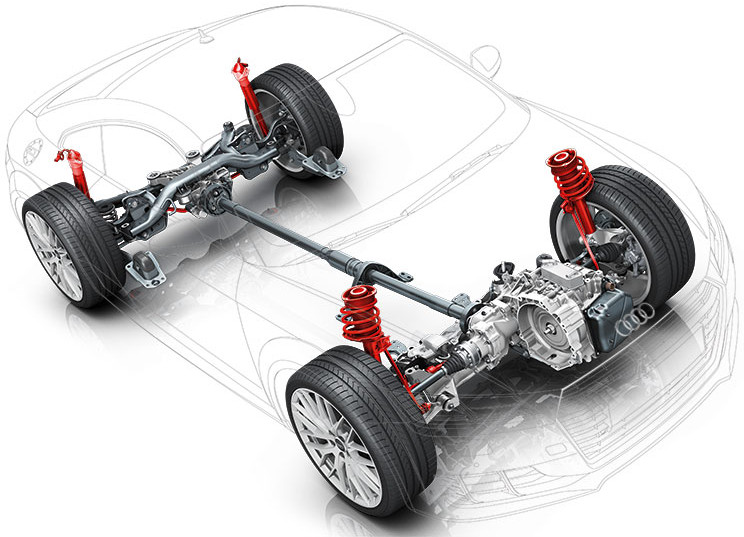
\includegraphics[width=\textwidth]{amortiguadores_AudiCoupeTT}
\end{minipage}



\item 
	\begin{minipage}[t][3.5cm]{0.75\textwidth}
	\textbf{Motor desbalanceado}
	Un motor eléctrico de \SI{15}{\kilo\gram} presenta un desbalance de su carga de \SI{20}{\gram} a \SI{125}{\milli\metre} de su eje.
	Se lo abulona a un soporte que limita su movimiento a la vertical.
	Para morigerar su vibración está amortiguado por cuatro resortes de \SI{40}{\kilo\newton\per\metre}, y un amortiguador de aceite con un coeficiente con lineal con la velocidad ajustado para que $c = 0.4 C_c$ ($C_c$, coeficiente de amortiguamiento crítico).

	Obtenga un rango aproximado de frecuencias de operación del motor en que la vibración es menor a \SI{0.2}{\milli\metre}.
\end{minipage}
\begin{minipage}[c][2cm][t]{0.2\textwidth}
	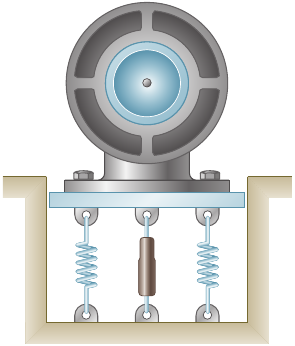
\includegraphics[width=\textwidth]{beer_fig_P19_144}
\end{minipage}



\item
\begin{minipage}[t][3.5cm]{0.75\textwidth}
	\textbf{leva}
	Las levas se caracterizan con los mapas de desplazamiento, que \emph{mapean} la función de su radio en un desplazamiento lineal del seguidor.
	La figura muestra como una leva con forma similar a un corazón permite que el desplazamiento de este último crezca y decrezca linealmente desde un pico.
				
	Asuma que en el pico el desplazamiento es de \SI{5}{\centi\metre} y en el mínimo es nulo, y que un motor hace que la leva describa $6\,\mathrm{rpm}$.  
	Suponiendo que este sistema se utiliza para forzar el sistema del ejemplo dado en clase, grafique el desplazamiento de $m$ en el estado estacionario en función del tiempo durante cuatro rotaciones de la leva.
\end{minipage}
\begin{minipage}[c][2cm][t]{0.2\textwidth}
	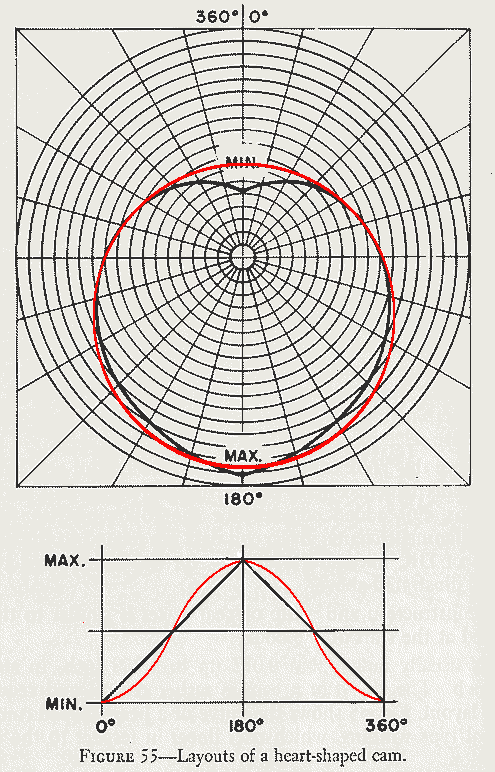
\includegraphics[width=\textwidth]{nok_wikkelmachine}
\end{minipage}




\end{enumerate}
\end{document}
